\chapter{Ondas --- Introdução}
\textsl{{\sffamily(Versão: \today)}}

\noindent
Neste capítulo faz-se uma introdução genérica do conceito de onda, e
introduzem-se as bases para o seu estudo (linguagem, descrições matemáticas e
propriedades dessas descrições). O conteúdo deste capítulo não é especificamente
a luz, mas os fenómenos ondulatórios em geral (som, ondas na superfície da água,
vibrações em sólidos, etc.). Mas não se pense, por isso, que se pode ``saltar''
diretamente para o Capítulo~3. A menos que o leitor domine já os conceitos e
métodos aqui introduzidos, os capítulos seguintes serão completamente
incompreensíveis.

\section{Propagação corpuscular e ondulatória}
A luz é, claramente, \emph{algo} que se propaga. Mas o que é esse \emph{algo},
ao certo, e como é que se propaga?

Podemos classificar os processos de propagação em dois tipos principais. Nos
processos ditos \emph{corpusculares}, a entidade propagada de um ponto do espaço
para outro é transportada por partículas materiais (ou seja, em última análise,
por átomos) que percorrem a totalidade do percurso entre os dois pontos.
Exemplos deste tipo de propagação são as correntes oceânicas, o vento, as
correntes dos rios, as correntes de conveção, os deslizamentos de terras e
avalanches, etc. Nestes exemplos, verifica-se a propagação de energia (térmica
e/ou cinética), de momento linear, de momento angular, de relações de
causalidade\footnote{Por exemplo, a fratura na superfície de uma placa de neve
consolidada no alto da montanha provoca uma avalanche que soterra um grupo de
montanhistas mais abaixo na encosta: a causa (fractura) e o efeito (tragédia dos
montanhistas) não ocorrem no mesmo lugar; logo a relação de causa-efeito teve
que viajar entre os dois sítios, teve que se \emph{propagar}.}, sempre
acompanhadas do movimento macroscópico de matéria (e é este movimento de matéria
que transporta as outras entidades propagadas que referi).

Mas há também a possibilidade da propagação de quantidades físicas ou relações
causais não ser acompanhada de movimento macroscópico de matéria. Por exemplo,
quando uma pedra cai na superfície calma de um lago, são originadas ondas de
forma circular que se propagam até às margens do lago, transportando 
energia e momento linear. A propagação destas ondas entre o ponto onde
a pedra cai e a margem não é acompanhada por uma corrente superficial da água.
Cada pequena porção de água na superfície do lago apenas sofre uma oscilação
vertical quando a onda passa. Outro exemplo: o som que se propaga desde um
instrumento musical até aos nossos ouvidos. O instrumento anima as camadas de
ar que lhe estão próximas de um movimento de vibração microscópico e esse
movimento de vibração vai sendo comunicado entre porções de ar contíguas até
estar em vibração a camada de ar que está encostada à membrana do tímpano nos
nossos ouvidos. Neste processo, apenas se propagou o estado de vibração, não
foi necessário que as moléculas de ar viajassem desde o instrumento musical até
nós. Este tipo de propagação, em que não há movimento significativo de matéria,
ou ainda, por outras palavras, que não é acompanhado por um correspondente
transporte de massa, chama-se propagação \emph{ondulatória}.

Dada a maneira como acabámos de classificar os fenómenos de propagação, podemos
agora recolocar a pergunta com que começámos este capítulo: a luz é um
fenómeno corpuscular ou um fenómeno ondulatório? Isto é, a luz consiste num
chuveiro de pequenas partículas que viajam desde as fontes de luz até aos
objetos iluminados e destes até aos nossos olhos, ou trata-se antes de uma
perturbação do valor de alguma propriedade do espaço ou do estado de vibração de
algum meio material que percorre esse trajeto, sem que haja um correspondente
deslocamento de qualquer tipo de partícula?

As primeiras respostas dadas a esta pergunta foram fornecidas por Huygens, em
1678, e por Newton, em 1704. Enquanto que o primeiro acreditava na natureza
ondulatória da luz, o segundo considerava-a constituída por partículas.

Note-se
que ambos apresentaram argumentos sólidos a favor das hipóteses que defenderam:
\begin{itemize}
\item
    Huygens entendia que a luz devia ser um fenómeno ondulatório porque não eram
    observados sinais de colisões entre as partículas de luz de dois feixes que
    se cruzavam; logo, dizia, essas partículas não existiam e, portanto, a luz
    só podia ser um fenómeno ondulatório. Para além disso, a hipótese
    ondulatória permitia explicar os fenómenos da óptica geométrica mais
    simplesmente do que a hipótese corpuscular;
\item
    Newton, por seu turno, notava que a luz se propaga em linha recta, ao
    contrário das ondas do mar ou do som. Além disso, uma propagação
    ondulatória (que tem na base, pensava ele, uma vibração da matéria) não
    deveria ser possível na ausência de matéria. Ora, como a luz das estrelas
    chega até nós depos de atravessar o vazio interestelar, ela não poderia
    assim ser um fenómeno ondulatório.
\end{itemize}
A opinião de Newton prevaleceu durante cerca de cem anos, até que, em 1801,
Thomas Young e Augustin-Jean Fresnel mostraram através de experiências de
interferência que a luz era com certeza um fenómeno ondulatório. Por outro
lado, em meados do séc.~XIX, James Clerk Maxwell, partindo das equações
fundamentais do electromagnetismo (que ele tinha ajudado a estabelecer), deduziu
uma equação de ondas que se propagam com a velocidade da luz. Deduziu assim que
a luz era uma onda electromagnética. Estas e outras descobertas afirmaram
incontestavelmente a hipótese ondulatória da luz.

Mas que resposta se dava à objecção de Newton? Ou seja, como é que a luz, sendo
uma onda, podia propagar-se no espaço interestelar? Das duas, uma: ou as ondas
de luz, ao contrário de todos os outros tipos de ondas então conhecidos, não
eram vibrações de um meio material, ou então o espaço interstelar não era
completamente vazio.  Os físicos dos sécs.~XVIII e~XIX foram-se progressivamente
convencendo desta última hipótesea; estavam convencidos  de que um fluido muito
pouco denso e muito pouco viscoso, a que foi dado o nome de \emph{éter
lumífero,} preenchia todo o universo, permeando mesmo os corpos materiais. As
vibrações dese fluido seriam a luz, assim como as vibrações atmosféricas
constituem o som. 

A hipótese da existência do éter era aceite pela generalidade dos físicos do
final do séc.~XIX. Lord Kelvin chegou mesmo a formular uma teoria atómica na
qual os átomos seriam turbilhões de éter. No entanto, todas as tentativas de
provar experimentalmente a sua existência falharam. Algumas experiências foram
planeadas e executadas tão cuidadosamente que, se o éter existisse mesmo, elas
teriam-no com toda a certeza verificado.

Este falhanço grave da teoria aceite só foi resolvido em 1905, por Einstein,
que abdicou da crença na existência de um meio material que desse suporte à
propagação da luz. A luz seria então uma vibração de um meio não material --- O
campo eletromagnético. O desenvolvimento desta ideia fez-se na chamada Teoria da
Relatividade Restrita, em que Einstein reformulou completamente as noções de
tempo e de espaço. Mas essa história fica para outra altura.

Vamos agora interromper o estudo da luz para introduzir algumas noções gerais
sobre ondas.

\section{Ondas}
Vejamos alguns exemplos de fenómenos ondulatórios, para ajudar a concretizar as
ideias que serão discutidas a seguir.
\begin{itemize}
\item \textbf{Ondas na superfície da água}\\
    Já todos observámos ondas na superfície de massas de água; por exemplo, as
    que se formam quando pedras caem num lago ou quando alguém mergulha numa
    piscina. Que \emph{coisa} se move quando a onda se propaga? Não é decerto a
    própria água, que se encontra essencialmente em repouso. As moléculas de
    água na superfície deslocam-se de facto quando a onda passa por elas, mas o
    seu movimento tem uma extensão muito pequena quando comparada com a do
    movimento da onda propriamente dita: esta percorre toda a superfície do
    lago, enquanto que aquelas oscilam apenas alguns milímetros para cima e para
    baixo, quando a onda passa pela região onde se encontram (veja a
    Figura~\ref{fig:20-010}).
    \begin{figure}[htb]
        {\centering
            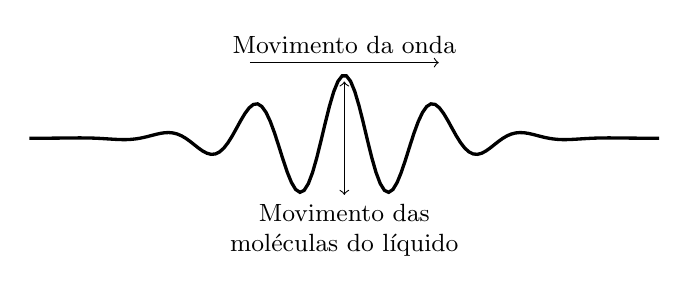
\begin{tikzpicture}[scale=0.8]
\small
\draw[very thick, domain=-5:5, variable=\x,samples=150] plot ({\x}, {cos(\x*250)*exp(-\x*\x*0.3)});
\draw [->] (-1.5,1.2) -- (1.5,1.2) node[midway,above]{Movimento da onda};
\draw [<->] (0,0.9) -- (0,-0.9) node[below, text width=3.5cm, align=center]
    {Movimento das moléculas do líquido};
\end{tikzpicture}

            \caption{Movimento da água na passagem de uma onda
                superficial.\label{fig:20-010}}

        }
    \end{figure}
    Em resultado deste movimento de oscilação vertical da água quando uma onda
    passa, a forma da superfície livre do líquido deixa de ser plana e
    horizontal, notando-se uma perturbação, uma sucessão localizada de pontos da
    superfície acima do nível médio e abaixo do nível médio. De facto, é essa
    perturbação na forma da superfície da água que constitui a onda.

    O que é que se move, então, quando uma onda se propaga na superfície da água
    de lago? É a própria perturbação na forma da superfície da água. 

    Assim, descrever matematicamente as ondas na superfície da água consiste,
    pois, em descrever a perturbação na forma da dessa superfície, e essa
    descrição pode ser feita utilizando uma função que depende do tempo e da
    posição sobre a superfíce, cujo valor é, em cada ponto e em cada instante, o
    do desnível desse ponto relativamente ao nível médio da superfície da água,
    em cada instante.

\item \textbf{Ondas de som}\\
    Quando um som se propaga num gás (por exemplo, em ar), as moléculas desse
    gás adquirem um movimento microscópico de oscilação coletiva (sobreposto ao
    movimento individual de agitação térmica), que se estabelece na direção de
    propagação do som. Por essa razão, no ar ficam definidas regiões de
    compressão e rarefação, que se alternam ao longo da direção da propagação
    (veja a Figura~\ref{fig:20-020}).
    \begin{figure}[htb]
        {\centering
            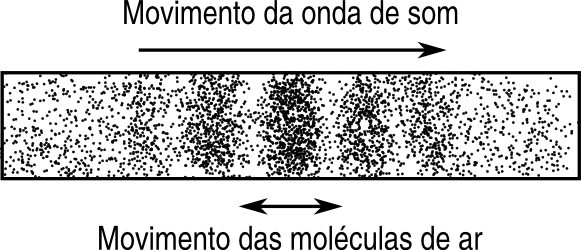
\includegraphics{figs/f20-020.png}
            \caption{Onda de som e movimento das moléculas de ar.%
                \label{fig:20-020}}

        }
    \end{figure}
    Como no caso das ondas na superfície da água, a \emph{coisa} que aqui se
    propaga ao longo do espaço não é, em rigor, coisa (material) nenhuma, são
    apenas as perturbações nos valores de algumas propriedades do ar (como a
    densidade ou a pressão) relacionadas com as compressões e rarefações
    inerentes à propagação do som. Também aqui devemos introduzir uma função
    (por exemplo, a pressão ou a densidade) cujo valor em cada ponto e em cada
    instante é o da perturbação que constitui a onda de som.

\item \textbf{Ondas numa corda esticada}\\
    Quando se dá um safanão brusco numa corda esticada horizontalmente,
    altera-se a forma da corda. Ela deixa de ser rectilínea\footnote{Na verdade,
    por causa do seu peso, uma corda esticada horizontalmente não assume uma
    forma rigorosamente retilínea, mas antes a forma de uma curva chamada
    \emph{cantenária,} que pode ser apreciada nos cabos de alta tensão, por
    exemplo.}, passando a apresentar uma curva pronunciada induzida pelo
    safanão, que se origina na vizinhança da extremidade agitada e que se
    propaga até à outra.

    De novo, nesta propagação de \emph{algo} ao longo de toda a extensão da
    corda, não ocorre o deslocamento de nenhuma porção de matéria de um dos
    extremos até ao outro. Nenhum segmento de corda se desloca acompanhando a
    propagação. Em vez disso, cada porção de corda apenas realiza algumas
    oscilações, transversais ao sentido da propagação, e de pequena amplitude em
    compa\-ração com a distância percorrida pela \emph{coisa} que se propaga. Na
    verdade, como nos casos anteriores, a entidade que viaja nesta propagação é
    a deformação da corda, a curva nela induzida pelo safanão. Mais uma vez, é
    necessário introduzir uma função para descrever matematicamente a onda,
    função essa que tem, em cada ponto da corda e em cada instante, o valor do
    desvio da corda, nesse ponto, relativamente à sua forma esticada em repouso
    (sem safanões).

\item \textbf{``Ondas'' de espetadores numa bancada de estádio}\\
Nos espetáculos com muitos espetadores é frequente formarem-se ``ondas''
nas bancadas, quando os espetadores numa secção da bancada se levantam
momentaneamente ergendo os braços e sentando-se logo a seguir, sendo
imediatamente imitados pelos que ocupam as secções contíguas, propagando-se esta
ação coletiva até ao extremo da bancada. Nenhum espetador tem que se levantar e
correr ao longo da bancada para que ocorra o movimento da ``onda''; cada
espetador apenas se levanta e se volta a sentar; mas isso é suficiente para que
``algo'' (a onda) viaje ao longo da bancada. Como nos exemplos anteriores, uma
descrição matemática da ``onda'' parte da introdução de uma função do tempo e do
espaço, função essa cujo valor, em cada ponto e em cada instante, indica se o
espetador com assento nesse ponto estava, nesse instante, levantado ou sentado.
\end{itemize}

\subsection{A função de onda $\psi(x,y,z,t)$}
Nos exemplos de processos ondulatórios que considerámos (e em \emph{todos} os
outros que omitimos), a descrição matemática do fenómeno passa pela introdução
de uma função do tempo e da posição, cujo valor é, em cada instante e em cada
ponto, o da perturbação que constitui a onda em análise. Essa função chama-se
\emph{função de onda} e representa-se normalmente pela letra grega $\psi$ (lê-se
``psi''). A natureza e propriedades gerais desta função (em particular, as
unidades em que é expresso o seu valor) dependem da natureza da onda: quando a
função de onda descreve um deslocamento (como nas ondulações da superfície dos
líquidos ou nas ondas em cordas), a função de onda tem dimensões de distância e
as suas unidades SI são, portanto, o metro. Mas há muitas situações em que a
onda é descrita por outras variáveis que não o deslocamento. Por exemplo, nas
ondas de som em ar, usa-se normalmente a pressão atmosférica para descrever a
perturbação ondulatória; nesses casos, a função de onda tem dimensões de
pressão (a unidade SI é o pascal, Pa). Outro exemplo comum é o das ondas
eletromagnéticas (como a luz) que são descritas pelas variações do campo
eléctrico; então as dimensões da função de onda são as do campo elétrico, e a
unidade SI é o volt por metro (V/m).

Uma onda é então uma perturbação relativamento ao valor médio (ou expectável, ou
de equilíbrio) de uma função característica de um dado sistema físico, que se
propaga no espaço. A Figura~\ref{fig:20-030} tenta ilustrar isso mesmo.
\begin{figure}[htb]
    {\centering
        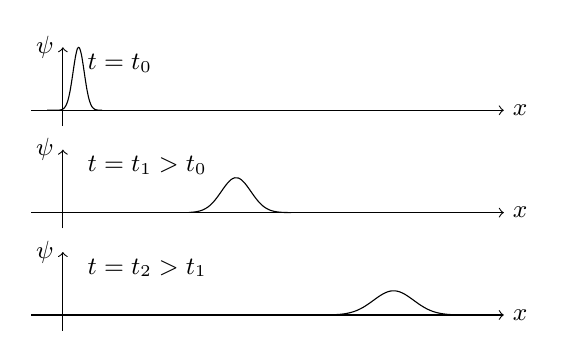
\begin{tikzpicture}
            \small
			\begin{scope}
            	\draw [->] (-0.4,0) --++(6,0) node [right]{$x$};
            	\draw [->] (0,-0.2) --++(0,1) node [left]{$\psi$};
				\pgfmathsetmacro{\t}{0}
				\draw[domain=\t-0.2:\t+0.5, smooth, samples=30,variable=\x]
					plot ({\x},{0.8/(0.4*\t+1)*exp(-100/(3*\t+1)*(\x-0.2-\t)^2)});
				\node at (0.2,0.6) [anchor=west] {$t=t_0$};
			\end{scope}
			\begin{scope}[yshift=-1.3cm]
            	\draw [->] (-0.4,0) --++(6,0) node [right]{$x$};
            	\draw [->] (0,-0.2) --++(0,1) node [left]{$\psi$};
				\pgfmathsetmacro{\t}{2}
				\draw[domain=\t-0.4:\t+0.9, smooth, samples=30,variable=\x]
					plot ({\x},{0.8/(0.4*\t+1)*exp(-100/(3*\t+1)*(\x-0.2-\t)^2)});
				\node at (0.2,0.6) [anchor=west] {$t=t_1>t_0$};
			\end{scope}
			\begin{scope}[yshift=-2.6cm]
            	\draw [->] (-0.4,0) --++(6,0) node [right]{$x$};
            	\draw [->] (0,-0.2) --++(0,1) node [left]{$\psi$};
				\pgfmathsetmacro{\t}{4}
				\draw[domain=\t-0.6:\t+1.1, smooth, samples=30,variable=\x]
					plot ({\x},{0.8/(0.4*\t+1)*exp(-100/(3*\t+1)*(\x-0.2-\t)^2)});
				\node at (0.2,0.6) [anchor=west] {$t=t_2>t_1$};
			\end{scope}
        \end{tikzpicture}\par
    }
    \caption{Propagação ao longo do eixo dos $x$ de uma perturbação no valor de
    uma função $\psi(x,t)$. À medida que o tempo passa, a região do espaço onde
    a função apresenta valores diferentes do de equilíbrio vai-se deslocando
    para a direita. A forma da onda neste exemplo não permanece
    constante: a região onde a perturbação está definida vai-se alargando e o
    seu valor máximo vai diminuindo.\label{fig:20-030}}
\end{figure}
Note-se que, se há propagação da perturbação, a função não pode ser constante
(se o for, tem em cada ponto um valor que não muda de instante para instante, ou
seja, não há movimento) nem homogénea (se o for, tem o mesmo valor em todos os
pontos, ou seja, o movimento não é observável). A função de onda deve pois ser
simultaneamente função da posição e do tempo.

\subsection{Equação de onda unidimensional}
Na propagação de uma onda, a forma da perturbação pode manter-se inalterada,
verificando-se apenas uma translação dessa perturbação no espaço com o passar do
tempo, ou pode acontecer que a sua forma se altere. Para dar dois exemplos, um
sinal luminoso propaga-se no vazio sem sofrer alterações (a menos que percorra
distâncias cosmologicamente significativas) no trajeto; mas um sinal sonoro
sofre alterações óbvias enquanto percorre em ar grandes distâncias\footnote{Um
exemplo muito claro deste efeito nota-se com trovões: o trovão de um relâmpago
que ``cai'' perto de nós parece um estalo muito intenso, súbito e breve; o de um
afastado é aquele típico ribombar grave e prolongado.}.  As propagações sem
alteração de forma são mais simples e, por isso, é nessas que nos iremos
concentrar. Veremos mais à frente que o formalismo que vai ser desenvolvido pode
ainda ser aplicado a propagações com alteração de forma. 

Vamos, para já, estudar o caso unidimensional (em que a função de onda depende
de apenas uma coordenada espacial, $x$, e do tempo), com menor complexidade
matemática. Consideremos então um sinal ondulatório que se propaga sem alteração
da forma com velocidade\footnote{Por ``velocidade'' ententenda-se aqui
``componente escalar da velocidade". Isto é, $v_x$ pode ser positivo, caso em
que a onda se propaga no sentido positivo do eixo dos $x$; ou pode ser negativo,
quando a onda se propaga no sentido negativo desse mesmo eixo.} $v_x$ ao longo
do eixo dos $x$, com função de onda $\psi(x,t)$. Dizer que a onda se propaga sem
alteração da forma é equivalente a dizer que os valores que a função de onda
apresenta num num dado instante são, num intervalo de tempo $\delta t$, todos
deslocados ao longo da reta dos $x$, sofrendo uma translação, igual para todos,
de $v\delta t$. Seja $\psi_0(x)=\psi(x,t_0=0)$ a forma da função de onda no
instante $t_0=0$. De acordo com o que acabámos de dizer, o valor que esta função
toma num ponto particular qualquer $x_0$ é transportado, no intervalo de tempo
$\delta t=t-t_0=t$, para o ponto $x=x_0+v_x\delta t$. Ou seja,
\begin{equation*}
  \psi(x_0+v_x\delta t,\,t)=\psi_0(x_0),
\end{equation*}
expressão que, escrita em função da coordenada $x$ do ponto final (e tendo em
conta a escolha $t_0=0$), toma a forma
\begin{equation}\label{eq:constformwave}
  \psi(x,t)=\psi_0(x-v_xt).
\end{equation}

Deduzimos esta igualdade considerando apenas que a função $\psi$ depende de $x$ e
$t$ de tal modo que os seus valores se movem de ponto para ponto, sem alteração
de forma, com o passar do tempo. Ela é, assim, satisfeita por todas as funções
com aquele comportamento.

%A Figura~\ref{fig:f060} mostra exemplos de uma propagação com e sem alteração de
%forma.
%\begin{figure}[htb]
%  {\centering
%    \begin{tikzpicture}
%      \small
%      \begin{axis}[domain=-2:10,
%                   height=6cm,
%                   width=8cm,
%                   ymax=1.2,
%                   xmin=-2,
%                   xmax=10,
%                   yticklabels={},
%                   xlabel=$x$ (m)
%                   ]
%        \addplot [samples=150,thick] {exp(-(0.5*x)^2};
%        \addplot [samples=150,dashed, thick] {exp(-(0.5*x-1)^2)};
%        \addplot [samples=150, dotted, thick] {exp(-(0.5*x-2)^2)};
%        \node at (axis cs:0.9,1.05) [rotate=30] {$t=0$};
%        \node at (axis cs:3.2,1.05) [rotate=30] {$t=1\,$s};
%        \node at (axis cs:5.2,1.05) [rotate=30] {$t=2\,$s};
%      \end{axis}
%      \begin{axis}[xshift=7.5cm,
%                   domain=-2:10,
%                   height=6cm,
%                   width=8cm,
%                   ymax=1.2,
%                   xmin=-2,
%                   xmax=10,
%                   yticklabels={},
%                   xlabel=$x$ (m)
%                 ]
%        \addplot [samples=150,thick] {exp(-(0.5*x)^2};
%        \addplot [samples=150,dashed,thick] {exp(-(0.5*x-1)^2/1.5)/1.25};
%        \addplot [samples=150,dotted,thick] {exp(-(0.5*x-2)^2/3.0)/1.50};
%        \node at (axis cs:0.9,1.05) [rotate=30] {$t=0$};
%        \node at (axis cs:3.2,0.85) [rotate=30] {$t=1\,$s};
%        \node at (axis cs:5.2,0.75) [rotate=30] {$t=2\,$s};
%      \end{axis}
%    \end{tikzpicture}\par
%  }
%  \caption{No gráfico da esquerda, está representada a função $\exp[-(x/2-t)^2]$
%    (SI)
%    nos instantes $t=0$, $t=1$\,s e $t=2$\,s. A perturbação descrita por esta
%    onda propaga-se sem alteração de forma com velocidade $v=2$\,m/s. No grafico
%    da direita, representa-se a função $exp[-(0,5x-t)^2/(1,5t)]/(1+t/4)$ (SI),
%    nos mesmos instantes. Esta função, claramente, propaga-se com alteração de
%    forma: à medida que o tempo passa, a sua amplitude vai diminuindo e a sua
%  largura vai aumentando.\label{fig:f060}}
%\end{figure}

Consideremos uma perturbação que se propaga sem alteração de forma com função de
onda $\psi(x,t)=\psi(x-v_xt)$. Seja $z=x-v_xt$. Então $\psi(x-v_xt)=\psi(z)$ e temos
\begin{align*}
    \pd{\psi}{x}&=\pd{z}{x}\td{\psi_0}{z}=\td{\psi_0}{z}&
    \frac{\partial^2\psi}{\partial x^2}&=\pd{z}{x}\td{}{z}\left(\pd{\psi_0}{x}
        \right)=\frac{\text{d}^2\psi_0}{\text{d}z^2}\\
    \pd{\psi}{t}&=\pd{z}{t}\td{\psi_0}{z}=-v_x\td{\psi_0}{z}&
    \frac{\partial^2\psi}{\partial t^2}&=\pd{z}{t}\td{}{z}\left(\pd{\psi_0}{t}
        \right)=v_x^2\frac{\text{d}^2\psi_0}{\text{d}z^2}
\end{align*}
Comparando as duas igualdades do lado direito concluímos que
\begin{equation}\label{eq:waveq}
    \frac{\partial^2\psi}{\partial x^2} =
        \frac{1}{v_x^2} \frac{\partial^2\psi}{\partial t^2}.
\end{equation}
Esta é a equação diferencial satisfeita pelas funções de onda das ondas
unidimensionais que se propagam sem alterações de forma, com velocidade
constante $v_x$ ao longo do eixo dos $x$. Chama-se, apropriadamente, \emph{equação
de onda unidimensional.} Os fenómenos ondulatórios atrás referidos (com a
exceção das ondas das bancadas de estádio, que são regidas por uma dinâmica mais
social do que física), quando reduzidos a uma dimensão, são descritos através
funções de onda que satisfazem a equação de onda unidimensional.


\subsection{O princípio da sobreposição}
Uma vez que a derivada (ou a dupla derivada) de uma combinação linear de funções
é igual à combinação linear correspondente das derivadas de cada
uma\footnote{Isto é,
    $\displaystyle\pd{}{x}(a_1\psi_1+a_2\psi_2+\ldots+a_n\psi_n)=
a_1\pd{\psi_1}{x}+a_2\pd{\psi_2}{x}+\ldots+a_n\pd{\psi_n}{x}.$}, então a soma
de duas soluções (ou a combinação linear de qualquer número de soluções) da
equação de onda é ainda uma solução da equação de onda. A esta propriedade das
ondas chama-se \emph{princípio de sobreposição.} Em termos práticos, isto
significa que quando numa região do espaço coincidem duas ondas com a mesma
natureza $\psi_1(x,y,z,t)$ e $\psi_2(x,y,z,t)$, o valor da perturbação
ondulatória resultante é igual, em cada ponto e em cada instante, à soma das
duas, isto é,
\begin{equation*}
\psi(x,y,z,t)=\psi_1(x,y,z,t)+\psi_2(x,y,z,t).
\end{equation*}

\section{Ondas sinusoidais}\label{sec:hamonicwaves}
As funções de onda podem ter formas muito variadas. Por exemplo, a
Figura~\ref{fig:20-cello} ilustra a forma como a pressão atmosférica varia com o
tempo em duas ondas de som, uma produzida por um diapasão, a outra por um
violoncelo, ambos a tocar a mesma nota (Lá 4).
\begin{figure}[htb]
{\centering
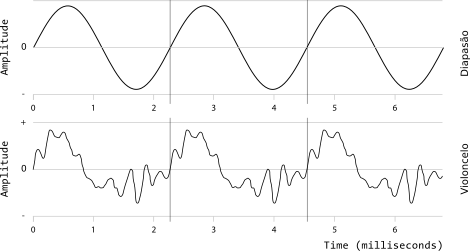
\includegraphics[width=0.5\linewidth]{figs/f20-cello.png}\par
}
\caption{Dependência da pressão atmosférica com o tempo, numa onda de som
produzida por um diapasão (em cima) e por um violoncelo (em baixo), ambos a
tocar a nota Lá 4. (Adaptado de
\protect\url{https://processing.org/tutorials/sound/})\label{fig:20-cello}}
\end{figure}
Apesar desta grande diversidade, é possível um tratamento relativamente
unificado das diferentes formas de onda porque se demonstra que qualquer função
fisicamente razoável se pode escrever como combinação de funções seno e cosseno.
A técnica matemática para construir essas sobreposições chama-se análise de
Fourier. Mais tarde estudaremos essa técnica em algum detalhe mas, para já, é
suficiente saber que ela existe e que, por isso, basta-nos estudar o
comportamento e propriedades das funções de onda com forma sinusoidal (isto é,
com a forma do seno ou do cosseno), pois qualquer outra função de onda pode ser
construída com sobreposições dessas funções.

Consideremos por enquanto o caso unidimensional, para introduzir pouco a pouco o
formalismo matemático. As ondas sinusoidais (que também são conhecidas como
\emph{ondas harmónicas} ou \emph{ondas monocro\-máticas}) unidimensionais são
funções da posição e do tempo com a forma genérica
\begin{equation}\label{eq:hwav}
    \psi(x,t)=A\cos\left(\frac{2\pi}{\lambda}\left[x-v_xt\right]+
            \varphi_0\right)
\end{equation}
Nesta equação $x$ e $t$ representam, respetivamente, a posição e o tempo, e
$v_x$ a componente escalar da velocidade de propagação da onda.\footnote{Recorde
que dizer que $v_x$ é a componente escalar da velocidade de propagação significa
dizer que é um número real que pode ser positivo (quando a propagação se faz no
sentido positivo do eixo dos $x$) ou negativo (quando se faz no sentido
oposto).}
Note-se que esta expressão para uma onda harmónica satisfaz a condição geral das
ondas que se propagam sem alteração da forma da eq.~\eqref{eq:constformwave}.

Os parâmetros que caracterizam a função de onda têm os nomes
\emph{amplitude} ($A$), \emph{comprimento de onda} ($\lambda$), e
\emph{constante de fase} ($\varphi_0$). A propósito, chama-se \emph{fase} da onda
ao argumento da função trignométrica, ou seja, à função da posição e do tempo
\begin{equation}\label{eq:harmonicphase}
\phi(x,t)=\frac{2\pi}{\lambda}(x-v_xt)+\varphi_0.
\end{equation}
Os argumentos das funções transcendentes (como é o caso da função cosseno) devem
ser adimensionais; assim, a fase de uma onda não tem dimensões, pelo que
$\lambda$ deve ser uma distância.  A amplitude tem as dimensões da função de
onda e, assim, depende da natureza da onda; pode ser uma distância (como nas
ondas do mar ou nas vibrações de uma corda esticada), mas pode também ter outras
dimensões, como já foi dito.

Vejamos o significado e o efeito de cada um destes parâmetros\footnote{O que a
seguir se afirma pode, \emph{e deve,} ser verificado com uma calculadora
gráfica ou uma folha de cálculo. Programe a forma da função de onda
substituindo os parâmetros $A$, $\lambda$, $v_x$ e $\varphi_0$ por valores
constantes à sua escolha e dando a $t$ um valor fixo; veja o que acontece para
valores de $t$ crescentes; veja o que acontece gráfico quando altera algum dos
parâmetros.}.
Na Figura~\ref{fig:20-050} apresentam\--se os gráficos de uma função harmónica
como função de $x$, em três instantes $t=0$ (linha contínua), $t=0,15$\,s (linha
a tracejado) e $t=0,3$\,s (linha a pontilhado). Na função de onda representada, os
valores dos parâmetros são $A=0,75$, $\lambda=1,5$\,m, $v_x=1,5$\,m/s e
$\varphi_0=0$.  Observando o gráfico, notamos que o valor da amplitude, $0,75$,
é o módulo dos extremos de variação da função; notamos também que a distância
entre os picos sucessivos da onda, num determinado instante, tem o valor que
atribuímos ao comprimento de onda $\lambda$.
\begin{figure}[htb]
{\centering
    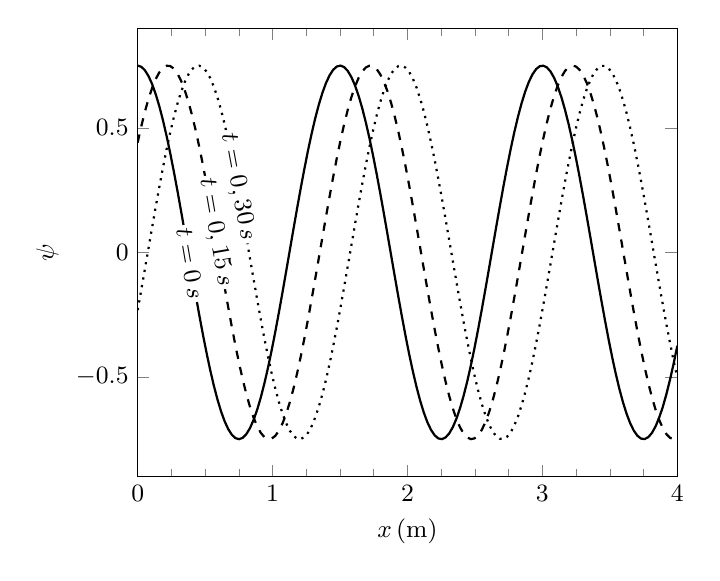
\begin{tikzpicture}
  \small
  \begin{axis}[domain=0:4,
               samples=150,
               xmin=0, xmax=4,
               no marks,
               xlabel=$x$\,(m), ylabel=$\psi$,
               xtick={0,1,2,3,4},
               minor x tick num={3}]
               \addplot [black,thick] {0.75*cos(deg(2*pi*x/1.5))}
            node [ pos=0.1, sloped, fill=white,inner sep=1] {$t=0\,s$};
        \addplot [black, dashed, thick]{0.75*cos(deg(2*pi*(x/1.5-0.15/1.0))}
            node [pos=0.13, sloped, fill=white,inner sep=1] {$t=0,15\,s$};
        \addplot [black, dotted, thick]{0.75*cos(deg(2*pi*(x/1.5-0.30/1.0))}
            node [pos=0.18, sloped, fill=white,inner sep=1] {$t=0,30\,s$};
  \end{axis}
\end{tikzpicture}
\par
}
\caption{Gráficos da função de onda
$\psi(x,t)=A\cos(2\pi[x-v_xt]/\lambda+\varphi_0)$, com $A=0,75$, $\lambda=1,5$,
$v_x=1,5$\,m/s e $\varphi_0=0$, para $t=0$ (linha a cheio), $t=0,15$\,s (linha a
tracejado) e $t=0,3$\,s (linha a pontilhado).\label{fig:20-050}}
\end{figure}
A figura também mostra que, à medida que o tempo avança, a função de onda
aparece deslocada cada vez mais para a direita: a perturbação sinusoidal
\emph{propaga-se}. Quanto tempo decorre entre a passagem de dois máximos
sucessivos num dado sítio? Esse é o intervalo de tempo necessário para a onda
percorrer uma distância igual ao seu comprimento de onda, ou seja, esperamos que
tenha o valor $\delta t=\lambda/|v_x|=1,0$\,s. Da figura, notamos que em 0,3\,s,
a onda avança 0,45\,m; proporcionalmente, avançará 1,5\,m em 1,0\,s, como
esperávamos. O tempo que decorre entre a chegada a um dado ponto de dois máximos
sucessivos (ou mínimos sucessivos ou, mais em geral, dois pontos com fase
equivalente sucessivos) chama-se \emph{período} da onda e é normalmente
representado com a letra $T$.  Desta análise concluímos o seguinte:
\begin{itemize}
\item
    a \emph{amplitude} de uma onda harmónica é o valor máximo dos desvios da
    função de onda relativamente ao seu valor médio. É a amplitude da oscilação;
\item
    o \emph{comprimento de onda} de uma onda harmónica é a distância entre
    máximos sucessivos dessa onda;
\item
    o \emph{período} $T=\lambda/|v_x|$ de uma onda harmónica é a duração do
    intervalo de tempo entre a passagem de dois máximos sucessivos da onda num
    ponto dado.
\end{itemize}
Falta discutir o significado da constante de fase $\varphi_0$. Este parâmetro está
relacionado com o valor inicial (para $t=0$) da onda na origem (em $x=0$).
Escolhendo, como fizemos acima, $\varphi=0$, resulta $\psi(x=0,\,t=0)=A$. Caso a onda
que queremos descrever se anulasse (por exemplo) no instante inicial e na
origem, escolheríamos $\varphi=\pi/2$. Para uma dada onda, podemos sempre escolher
$\varphi_0=0$ definindo de forma conveniente as origens espacial e temporal. Para
além disso, podemos escolher a função seno ou a função cosseno na descrição da
onda, ajustando convenienemente o valor da constante de fase, dado que $\sin
x=\cos(x-\pi/2),\ \forall x\in \mathbb{R}$. Ou seja, enquanto que a amplitude, o
comprimento de onda e a velocidade de propagação de uma onda são propriedades da
onda em si, o valor da constante de fase depende também de escolhas que cada um
faz mais ou menos arbitrariamente.
 
A \emph{frequência} de uma onda sinusoidal é o número de máximos da onda que
atingem um determinado ponto por unidade de tempo. Assim, a frequência é o
inverso do período:
\begin{equation*}
    f=\frac{1}{T}=\frac{|v_x|}{\lambda}.
\end{equation*}
A frequência exprime-se no SI em \emph{ciclos por segundo,} grandeza a que se dá
o nome de \emph{hertz} (Hz).

Seja $v=|v_x|$ o módulo da componente escalar da velocidade e $s=v_x/v=\pm1$ o
seu sinal. Fisicamente, $v$ traduz a rapidez com que a onda se propaga e $s$ o
sentido em que a propagação se dá. Obviamente, temos
\begin{equation*}
v_x=sv,\qquad\text{ com }s^2=1.
\end{equation*}
Usando estas igualdades na expressão da fase da eq.~\eqref{eq:harmonicphase},
podemos reescrevê-la como
\begin{align}
    \phi(x,t)&=\frac{2\pi}{\lambda}(s^2x-svt)+\varphi_0=
    \frac{2\pi}{\lambda}s(sx-vt)+\varphi_0\nonumber\\
&=s(k_xx-\omega t)+\varphi_0,\label{eq:hrmonicphase}
\end{align}
onde
\begin{equation}
k_x=\frac{2\pi}{\lambda}s
\end{equation}
é um número real positivo ou negativo que pode ser interpretado como a
componente escalar de um vetor que tem o sentido da propagação da onda (o seu
sinal é igual ao de $v_x$), a que se dá o nome de \emph{vetor de onda}, e
\begin{equation}
\omega=\frac{2\pi}{\lambda}v=\frac{2\pi}{T}=2\pi f
\end{equation}
é um real positivo chamado \emph{frequência angular}, que mais não é que a
frequência da onda, expressa em radianos por segundo em vez de em ciclos por
segundo. Substituindo agora a expressão da fase da eq.~\eqref{eq:hrmonicphase}
na função de onda da eq.~\eqref{eq:hwav}, obtemos
\begin{equation*}
\psi(x,t)=A\cos(s[k_xx-\omega t] +\varphi_0),
\end{equation*}
e podemos ``deixar cair'' o sinal $s$ ajustando convenientemente
o valor da constante de fase, resultando uma forma muito usual
(bastante mais frequente que a da eq.~\eqref{eq:hwav}) da expressão da função de
onda harmónica sinusoidal:
\begin{equation}\label{eq:hwav2}
\psi(x,t)=A\cos([k_xx-\omega t] +\varphi_0).
\end{equation}

Para completar esta já longa secção sobre a representação matemática das funções
sinusoidais, deixo como exercício a demonstração da equivalência com as
eqs.~\eqref{eq:hwav} e~\eqref{eq:hwav2} de uma terceira expressão para as ondas
sinusoidais:
\begin{equation*}
\psi(x,t) = A\cos\left(2\pi\left[\frac{x}{\lambda}\pm\frac{t}{T}\right]+\varphi_0
\right),
\end{equation*}
onde os vários símbolos têm o significado já introduzido e o sinal a tomar no
parentesis reto é o oposto ao de $v_x$.



%Frequentemente, a função de onda harmónica encontra-se parametrizada numa forma
%alternativa à apresentada na eq.~\eqref{eq:hwav}:
%\begin{equation*}
%  \psi(x,t)=A\cos\left(kx\pm\omega t+\phi_0\right).
%\end{equation*}
%Os parâmetros $k$ e $\omega$, chamados respetivamente \emph{vetor de
%onda}\footnote{Mas em discussões unidimensionais é mais comum a designação de
%\emph{número de onda.}} e \emph{frequência angular,} relacionam\-\mbox{-se} com o
%comprimento de onda e com o período como
%\begin{align*}
%  k&=\frac{2\pi}{\lambda}&\omega=\frac{2\pi}{T}=2\pi f.
%\end{align*}
%O primeiro destes parâmetros representa a taxa espacial de variação da fase
%(\emph{quanto é que a fase varia por unidade de comprimento, num dado instante});
%a segunda, representa a taxa temporal de variação da fase (\emph{quanto é que a
%fase varia por unidade de tempo, num dado local}).
%
%Podemos calcular facilmente a velocidade de propagação de uma onda harmónica
%dividindo o seu comprimento de onda pelo tempo que ela demora a percorrer essa
%distância, ou seja, pelo seu período:
%\begin{equation*}
%  v=\frac{\lambda}{T} = \lambda f=\frac{\omega}{k}.
%\end{equation*}

\section{Representação complexa de ondas sinusoidais}
\subsection{Números complexos}
Seja \iu~um número não real a que chamamos \emph{unidade imaginária,} definido
como
\begin{align*}
  \iu&=\sqrt{-1}&\iu^2&=-1.
\end{align*}
Chamamos \emph{número imaginário} ao produto da unidade imaginária por um número
real e \emph{número complexo} à soma de um número real e de um número
imaginário:
\begin{alignat*}{3}
  \iu a,  &&\quad   a\in\mathbb{R} & \qquad &&\text{número imaginário}\\
  a+\iu b,&&\quad a,b\in\mathbb{R} & \qquad &&\text{número complexo}
\end{alignat*}
O conjunto de todos os números complexos representa-se pelo símbolo
$\mathbb{Z}$. Dado um número complexo ${z}=a+\iu b$, chamamos \emph{parte
real} à sua parcela real e \emph{parte imaginária} ao número real que é
multiplicado pela unidade imaginária:
\begin{equation*}
  {z}=a+\iu b,\quad a,b\in\mathbb{R} \quad \Rightarrow
  \begin{cases}
    \Re( z) &= a\qquad\text{parte real de } z\\
    \Im( z) &= b\qquad\text{parte imaginária de } z
  \end{cases}
\end{equation*}

O \emph{complexo conjugado} de um número complexo é o número complexo que se
obtém ao trocar o sinal à sua parte imaginária:
\begin{equation*}
   z = a+\iu b,\qquad a,b\in\mathbb{R}:\qquad  z^*=a-\iu b.
\end{equation*}

Um número complexo tem dois graus de liberdade reais independentes (as suas
partes real e imaginária). Nesse aspeto, é como um vetor de um espaço
bidimensional e, nesse sentido, pode ser representado como um ponto num plano
chamado \emph{plano complexo} (ou \emph{plano de Argand}), cujas coordenadas
cartesianas são as partes real e imaginária do número
\begin{figure}[htb]
  {\centering
    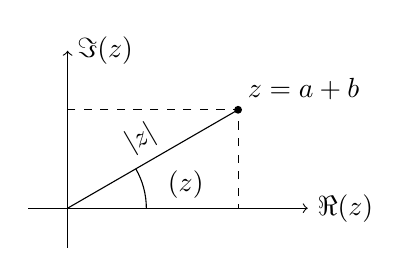
\begin{tikzpicture}
      \draw [->] (-0.5,0) -- +(3.55,0) node[right] {$\Re( z)$};
      \draw [->] (0,-0.5) -- +(0,2.5) node[right] {$\Im( z)$};
      \fill (30:2.5) circle(0.05) coordinate (z) node[above right]
        {$ z=a+\iu b$};
        \draw [thin, dashed] (0,0) -| (z) -- (z) -- (z)-|(0,0);
        \draw (0,0) --(z) node [midway, above, sloped] {$| z|$};
        \draw (30:1.0) arc(30:0:1.0) node [above,xshift=5mm]{$\Arg( z)$};
    \end{tikzpicture}\par
  }
  \caption{Plano de Argand. Cada número complexo é representado por um ponto
    cujas coordenadas cartesianas são as suas partes real e
  imaginária.\label{fig:argplane}}
\end{figure}
O \emph{módulo} de um número complexo é a distância que o separa da origem no
plano complexo, ou seja,
\begin{equation*}
   z = a+\iu b \Rightarrow | z|= \sqrt{a^2+b^2}=\sqrt{z\,z^*}.
\end{equation*}
Chama-se \emph{argumento} de um número complexo ao ângulo que o segmento que o
une à origem no plano complexo faz com o eixo real. Assim,
\begin{equation*}
   z = a+\iu b \Rightarrow \Arg( z)=\arctan\frac{b}{a},\quad
  \text{(mas atenção aos sinais e quadrantes).}
\end{equation*}
O módulo e o argumento de um número complexo podem, assim, ser vistos como as
coordenadas polares dos pontos que representam os números complexos no plano
complexo.

\subsection{Operações algébricas elementares}
As operações algébricas com números complexos seguem as mesmas regras que as
operações com números reais, complementadas com a da definição da unidade
imaginária, $\iu^2=-1$. Assim, dados $ u=a+\iu b$ e $ z=c+\iu d$,
\begin{description}
  \item[produto com um real]
    \begin{align*}
      \text{se }x\in\mathbb{R},\ x u&=x(a+\iu b)=xa+\iu xb;
    \end{align*}
  \item[adição/subtração] 
    \begin{align*}
       u\pm z &= (a+\iu b)\pm(c+\iu d) = (a\pm c) + \iu(b\pm d);
    \end{align*}
  \item[multiplicação]
    \begin{align*}
       u \,  z &= (a+\iu b)(c+\iu d)=\\
                           &=ac+\iu ad+ \iu bc+\iu^2 bd=(ac-bd)+\iu(ad+bc);
    \end{align*}
  \item [divisão] esta operação faz-se em dois passos: multiplica-se o numerador
    e o denominador pelo complexo conjudado do denominador; deste modo,
    transforma-se o denominador num número real (o quadrado do módulo do
    denominador original) e usa-se a primeira regra para completar o cálculo:
    \begin{align*}
      \frac{ u}{ z} &= 
        \frac{ u}{ z}\frac{ z^*}{ z^*}=
        \frac{ u  z^*}{|z|^2}\\
        &=\frac{(ac+bd)+\iu(bc-ad)}{c^2+d^2}
    \end{align*}
\end{description}

\subsection{Fórmula de Euler}
Considere a função complexa de uma variável real ($t\in\mathbb{R}$)
\begin{equation*}
  f(t) = \text{e}^{-\iu t}\left(\cos t+\iu \sin t\right),\qquad f(0)=1.
\end{equation*}
A derivada de $f$,
\begin{equation*}
  f'(t) = -\iu\e^{-\iu t}(\cos t+\iu \sin t)+
  \e^{-\iu t}(-\sin t+\iu \cos t)=0,
\end{equation*}
é identicamete nula, pelo que $f(t)$ é uma função constante. Uma vez que
$f(0)=1$, concluímos que $f(t)=1\ \forall t$, ou seja,
\begin{equation*}
  \e^{\iu t}=\cos t+i\sin t.
\end{equation*}
Esta fórmula chama-se \emph{Fórmula de Euler}.

Usando a fórmula de Euler é possível uma outra representação dos números
complexos. Dado um número complexo arbitrário $ z=a+\iu b$, considere-se o
número $ u = | z|\exp\left[\iu\Arg( z)\right]$. De
acordo com a fórmula de Euler, 
\begin{align*}
  \Re( u)&=| z|\cos[\Arg( z)]=a\\
  \Im( u)&=| z|\sin[\Arg( z)]=b,
\end{align*}
ou seja, os dois números $ z$ e $ u$ são iguais e as duas expressões
$a+\iu b$ e $| z|\exp(\iu\theta)$, com
$| z|=\sqrt{a^2+b^2}$ e $\theta=\arctan(b/a)$, são representações
equivalentes desse número.

\subsection{A representação de funções sinusoidais}
\label{sec:complexharm}
A representação complexa de funções sinusoidais consiste em fazer a substituição
\begin{equation*}
  \cos\phi \rightarrow \e^{\iu \phi}.
\end{equation*}
Claro que, nesta substituição, estamos a introduzir uma quantidade imaginária
($\iu\sin\phi$) que não estava presente na expressão inicial. Mas, em muitos
cálculos com interesse na física, essa parte imaginária ilegitimamente
introduzida não afeta a parte real, que representa a variável física relevante.
Nessas condições, não incorremos em erro com este procedimento, desde que no
final tomemos a parte real do resultado, descartando assim a parte imaginária
que não nos interessa. Assim, no caso da função de onda, iremos frequentemente
representá-la como
\begin{equation*}
  \psi(x,t)=A\cos(kx-\omega t+\varphi_0)
    \stackrel{!}{=}A\e^{\iu(kx-\omega t+\varphi_0)}
\end{equation*}
onde o símbolo $\stackrel{!}{=}$ indica que apenas a parte real da expressão no
lado direito deve ser considerada na igualdade. Daqui para a frente, esse
cuidado será subentendido, pelo que não voltaremos a usar este símbolo.

A representação complexa das ondas sinusoidais é usada porque simplifica imenso
algumas operações analíticas. Por exemplo, as derivações em ordem a $t$ ou em
ordem a $x$ de uma onda harmónica traduzem-se simplesmente na multiplicação por
um fator:
\begin{align*}
  \pd{}{t}\psi(x,t)&=-\iu\omega\psi(x,t)\\
  \pd{}{x}\psi(x,t)&=\iu k\psi(x,t).
\end{align*}

A representação complexa de funções periódicas é válida desde que não se
realizem operações em que a parte imaginária da representação (que é descartada
no final) ``infeta'' a parte real (que se toma no final dos cálculos como
resultado). As operações válidas incluem o produto com funções ou números reais, a adição e
subtração com funções ou números complexos e as derivações e integrações em
variáveis reais. As inválidas incluem produtos com números ou funções complexas.
No estudo das ondas em geral, e da óptica em particular, as operações mais
frequentemente realizadas são da primeira espécie, ``legais''. Quando for
necessário realizar cálculos envolvendo operações ``ilegais'', teremos que
reverter para a representação trignométrica. (Sempre que isso acontecer nestes
apontamentos, será feita a devida chamada de atenção.)

\section{Ondas em três dimensões. Frentes de onda}
Até agora, considerámos apenas ondas unidimensionais, isto é, cuja fase depende
apenas de uma coordenada e do tempo. Estas ondas são apropriadas para descrever
alguns fenómenos, como as ondas de vibração numa mola eástica, as ondas
transversais de vibração nas cordas das guitarras, ou a propagação do som num
tubo estreito, como uma mangueira ou uma flauta. Mas a fase das ondas de luz
proveniente de uma lâmpada depende das três coordenadas espaciais $x$, $y$ e
$z$. Como descrever ondas 3D como estas?



\subsection{Frentes de onda}
\subsubsection*{Superfícies de nível de funções do espaço}
Como discutimos na Secção~\ref{sec:surfgraf}, as funções contínuas de duas
variáveis $x$ e $y$ podem ser representadas graficamente pelas chamadas
\emph{curvas de nível}, linhas do plano $xy$ nas quais a função tem valor
uniforme. Encontramos estas curvas em cartas topográficas para indicar a
altitude do terreno, ou em cartas meteorológicas, normalmente para representar a
pressão atmosférica ou a temperatura. Do mesmo modo, as funções de três
variáveis $x$, $y$ e $z$ são caraterizadas por \emph{superfícies de nível,}
formadas por pontos onde a função apresenta um mesmo valor. Por exemplo, as
superfícies de nível do potencial gravítico na vizinhança da superfície
terrestre ($U=g(z-z_0$)) são planos horizontais; as da intensidade luminosa
(veremos mais tarde como se define, mas para já serve a noção intuitiva) em
torno da chama de uma vela têm forma aproximadamente esférica, com centro na
chama.

\subsubsection*{Frentes de onda são superfícies de nível da função de onda}
A função de onda $\psi(x,y,z,t)$ de um fenómeno ondulatório é tambem uma função
do espaço. Chamamos às suas superfícies de nível \emph{frentes de onda.} Como a
onda se propaga (ou seja, mais matematicamente, como a função de onda depende
também do tempo $t$) as suas superfícies de nível (ou seja, as frentes de onda)
vão-se modificando, deformando, ampliando, deslocando, à medida que o tempo
passa.

As frentes de onda das ondas que se formam na superfície de um lago calmo quando
nela cai uma pedra têm forma circular, com centro no ponto da superfície onde a
pedra caiu; as das ondas de choque de uma explosão aérea têm forma esférica, com
centro no ponto onde a explosão se deu; as das ondas de luz produzidas por uma
fonte luminosa muito afastada são também esféricas, mas o seu raio é tão elevado
que, para muitos efeitos, é como se fossem planas\footnote{Tal como a superfície
  da Terra: é esférica mas, como o seu raio (6400\,km) é muito maior do que as
  distâncias a que estamos acostumados no dia a dia, quase sempre pensamos nela
como plana.}. Qualificamos frequentemente as ondas com a forma das suas frentes
de onda; assim, chamamos ondas esféricas às que têm frentes de onda esférica,
ondas planas aquelas cujas frentes de onda são planas, etc. A
Figura~\ref{fig:oof040} ilustra algumas porções de frentes de onda de uma onda
plana (à esquerda) e de frentes de onda de uma onda esférica (à direita).
\begin{figure}[htb]
  {\centering
    \tdplotsetmaincoords{60}{125}
    \begin{tikzpicture}[tdplot_main_coords]
      \small
      \coordinate (O) at (0, 0, 0);

      \draw[-latex] (O) -- (1.5, 0, 0);
      \draw[-latex] (O) -- (0, 1.5, 0) node[pos = 1.1] {\(y\)};
      \draw[-latex] (O) -- (0, 0, 1.5) node[pos = 1.1] {\(z\)};

      \foreach \x in {0.0, 0.5, 1.0, 1.5} {%
        \draw[fill=gray!50, opacity = .8]
              (\x, -1, -0.9) -- (\x,  1, -1)
           -- (\x,  1,  1) -- (\x, -1,  0.9) -- cycle;}
      \draw [-latex] (1.5,0,0) -- (3.5,0,0) node[pos = 1.15] {\(x\)};
      \draw [-latex] (1.0,-1.1,1.1) -- (2.0, -1.1, 1.1) node [left] {$\vec v$};
    \end{tikzpicture}
    \hspace{1cm}
%%%%%%%%%%%%%%%%%%%%%%%%%%%%%%%%%%%%%%%%%%%%%%%%%%%%%%%%%%%%%%%%%%%%%%%%%%%%%%%%
    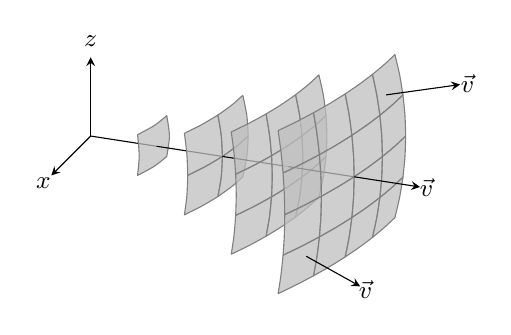
\begin{tikzpicture}[x=(225:0.707cm),y=(0:1cm),z=(90:1cm), >=stealth]
      \tikzset{cs/3d/.code args={#1:#2:#3}{%
      \pgfpointxyz{(#1)*sin(#2)*cos(#3)}{(#1)*sin(#2)*sin(#3)}{(#1)*cos(#2)}}}
      \tikzdeclarecoordinatesystem{3d}{\tikzset{cs/3d={#1}}}%     
      \tikzset{spherical patch/.style args={#1:#2:#3:#4}{insert path={
      [smooth, samples=3, line join=round]
      plot [domain=0:#3] (3d cs:{#4}:{#1+\x}:{#2}) --
      plot [domain=0:#3] (3d cs:{#4}:{#1+#3}:{#2+\x}) --
      plot [domain=#3:0] (3d cs:{#4}:{#1+\x}:{#2+#3}) --
      plot [domain=#3:0] (3d cs:{#4}:{#1}:{#2+\x}) -- cycle}}}
      \small
      \draw [->] (0,0)--(225:0.707cm) node[pos=1.2]{$x$};
      \draw [->] (0,0)--(90:1cm) node[pos=1.2]{$z$};
      \def\k{75} \def\j{90}
      \foreach \i [evaluate={\z=30/(\i+1); \p=\i; \q=(\i+1);}] in {0, 1, 2, 3}{
        \draw [-] (3d cs:\p:\j:\k) -- (3d cs:\q:\j:\k);
          \foreach \t in {0,...,\i}\foreach \a in {0,...,\i}
            \draw [gray, fill=gray!50, fill opacity=0.75, 
                   spherical patch={75+\t*\z:60+\a*\z:\z:\q}];
      }
      \draw [->] (3d cs:4:\j:\k) -- (3d cs:5:\j:\k) node[pos=1.1]{$\vec v$};  
      \def\k{85} \def\j{80}
      \draw [->] (3d cs:4:\j:\k) -- (3d cs:5:\j:\k) node[pos=1.1]{$\vec v$};  
      \def\k{65} \def\j{100}
      \draw [->] (3d cs:4:\j:\k) -- (3d cs:5:\j:\k) node[pos=1.1]{$\vec v$};  
    \end{tikzpicture}
%%%%%%%%%%%%%%%%%%%%%%%%%%%%%%%%%%%%%%%%%%%%%%%%%%%%%%%%%%%%%%%%%%%%%%%%%%%%%%%%
    \caption{Diferentes frentes de onda (ou a mesma frente, representada em
      instantes diferentes) de uma onda plana que se propaga na direção do eixo
      dos $x$ (à esquerda). À direita apresentam-se diferentes frentes de onda
      (ou a mesma frente de onda em diferentes instantes de uma onda esférica.
      Note que em diferentes pontos da frente de onda de ma onda esférica, a
      direção de propagação é diferente. ({\small\textsf{A imagem da direita foi
          adaptada de uma apresentada num post no \LaTeX{} Stack Exchange,
          disponível em
      \protect\url{http://tex.stackexchange.com/questions/262015/drawing-wave-propagation-using-tikz}}.})
      \label{fig:oof040}}\par
  }
\end{figure}
Note-se que cada porção da frente de onda propaga-se na direcção que lhe é
perpendicular. Assim, as duas representações na Figura~\ref{fig:oof040} podem
também interpretar-se como representações das \emph{mesmas} frentes de onda, em
diferentes instantes.

\subsection{Função de onda de ondas planas sinusoidais}
As ondas planas têm frentes de onda planas. Por definição de frente de onda, o
valor da função de onda em todos os pontos de uma mesma frente de onda é
o mesmo. Então, a função de onda depende da posição apenas pela variação com a
posição \emph{ao longo} da direção perpendicular às frentes de onda, ou seja, ao
longo da direção de propagação.

Consideremos uma onda plana harmónica com comprimento de onda $\lambda$,
frequência angular $\omega$, constante de fase $\varphi_0$ e amplitude $A$, e seja
$\hat k$ um vetor unitário com a direção e sentido da propagação. Dizer que
onda é plana e que a orientação da propagação é a do versor $\hat k$ significa
dizer que as suas frentes de onda são planas, perpendiculares a $\hat k$ e que
o seu movimento tem a orientação de $\hat k$. Logo, como discutimos no parágrafo
anterior, a função de onda depende do espaço apenas pela dependência da
coordenada orientada ao longo de $\hat k$. Seja $q$ essa coordenada (ver a
Figura~\ref{fig:f050}).  Por outro lado, dizer que esta onda é harmónica
significa que tem uma forma geral que se pode escrever como
\begin{equation}\label{eq:eq0}
  \psi(x,y,z,t)=A\cos\left(kq-\omega t+\varphi_0\right),
\end{equation}
com $k=2\pi/\lambda$. Seja $P$ um ponto de uma das frentes de onda, e
$\vec r=(x,y,z)$ o seu vetor posição. O valor da coordenada $q$ para este ponto
é facilmente calculado como
\begin{figure}[htb]
  {\centering
    \begin{tikzpicture}
      \small
      \draw[thin,->] (-0.2,0) -- (0.75,0) node[below] {$x$};
      \draw[thin,->] (0,-0.2) -- (0,0.75) node[left] {$y$};
      \coordinate (o) at (0,0);

      \foreach \d in {2.5, 3.0, 2.0} {
        \draw [thick,gray,name path=wf](10:\d)+(100:1.35)--+(280:0.8);
      }

      \path [name path=r] (o) -- (35:3);
      \path [name intersections={of=r and wf}];
      \coordinate (p) at (intersection-1);
      \draw [->] (o) -- ($(o)!0.99!(p)$) node[shift={(-2mm,0.5mm)}] {$\vec r$};
      \draw [->] (p) --+(10:0.85) node [yshift=-0.4cm] {$\vec k$};
      \draw [thin, dashed] (p) --+ (35:0.75);

      \draw (o)+(10:0.6) arc(10:35:0.6) node [shift={(2.0mm,-0.5mm)}]{$\theta$};
      \draw (p)+(10:0.6) arc(10:35:0.6) node [xshift=2.5mm]{$\theta$};
      \draw [thin, ->] (o) -- (10:3.5) node [above] {$q$};
    \end{tikzpicture}\par
  }
  \caption{\label{fig:f050}Onda plana monocromática que se propaga na direção de
    um vetor unitário $\hat k$. O eixo coordenado da coordenada $q$ está
    orientado segundo a direção de propagação. Em cada frente de onda, o valor
  de $q$ é uniforme.}
\end{figure}
\begin{equation*}
  q = r\cos\theta = \hat k\cdot\vec r,
\end{equation*}
onde $\theta$ é o ângulo entre $\vec r$ e $\vec k$.  Definindo o vetor (já não
unitário) $\vec k=2\pi/\lambda\,\hat k$, chamado \emph{vetor de
onda}\footnote{O vetor $\vec k$ é a versão tridimensional da
variável $k_x$ definida na Secção~\ref{sec:hamonicwaves}, a que demos o mesmo
nome. Obviamente, $k_x$ é a componente $x$ do vetor $\vec k$ agora introduzido.}
o produto $ks$ que aparece na expressão da fase na eq.~\eqref{eq:eq0} pode então
escrever-se como função das coordenadas do ponto $P$ na forma
\begin{equation*}
  kq=k\hat k\cdot \vec r=\vec k\cdot\vec r.
\end{equation*}
Por fim, substituindo na eq.~\eqref{eq:eq0}, obtemos a forma geral de uma onda
plana harmónica com vetor de propagação $\vec k$:
\begin{equation} \label{eq:plwav}
\psi(x,y,z,t)=A\cos(\vec k\cdot\vec r-\omega t+\varphi_0)
\end{equation}

Como exercício, considere o caso em que a onda se propaga ao longo do eixo dos
$x$. Como as frentes de onda são perpendiculares à direção de propagação, elas
devem ser planos paralelos ao plano $yz$, planos com $x$ constante. Então a fase
(que é constante em cada frente de onda) só pode depender de $x$\footnote{A
  coordenada que neste problema está alinhada com a direção de propagação é a
coordenada $x$. $x$ desempenha agora o papel da coordenada $s$.}, ou seja,
tratando-se de uma onda harmónica, a função de onda fica com a forma da
eq.~\eqref{eq:hwav}. Considere agora a expressão da eq.~\eqref{eq:plwav}; dado
que $\vec k$ tem a orientação da propagação (recorde que estamos a considerar em
que ela se faz segundo o sentido do eixo dos $x$), a única componente não nula
deste vetor é a primeira, que deve ter o valor $k=2\pi/\lambda$. Isto é, $\vec
k=(k,0,0)$; logo, $\vec k\cdot\vec r=kx$.  Substituindo este resultado na
expressão da eq.~\eqref{eq:plwav} obtemos justamente a forma unidimensional das
ondas sinusoidais da eq.~\eqref{eq:hwav}.

Naturalmente, a versão desta função de onda em representação complexa é
\begin{equation}\label{eq:phwfexp}
  \psi(\vec r,t)=A\e^{\iu(\vec k\cdot \vec r-\omega t+\varphi_0)}.
\end{equation}

\subsubsection{Equação de onda para ondas planas em três dimensões}
De acordo com a discussão precedente, ondas planas que se propagam na direção de
um vetor $\vec k$ têm frentes de onda perpendiculares a $\vec k$ e, assim sendo,
a sua dependência da posição $\vec r$ é feita através da combinação $\vec
k\cdot\vec r$. Se, para além de serem planas, se movem uniformemente sem
alteração da sua forma, então as coordenadas $\vec r$ e o tempo aparecem na
expressão da função de onda na combinação $\vec r-\vec vt$. Juntando tudo,
concluímos que uma onda plana que se propaga sem alteração de forma com
velocidade uniforme $\vec v$ na direção de um vetor $\vec k$ tem uma função de
onda com uma forma geral do tipo
\begin{equation}\label{eq:gpwwf}
  \psi(\vec r,t)=\psi\left(\vec k\cdot[\vec r-\vec vt]\right),
\end{equation}
onde $\vec v$ e $\vec k$ têm a mesma orientação. Seja agora $u=\vec k\cdot[\vec
r-\vec vt]$. É fácil verificar as igualdades
\begin{align*}
  \pd{\psi}{x_i}&=k_i\td{\psi}{u}&
  \pdd{\psi}{x_i}&=k_i^2\tdd{\psi}{u}\\
  \pd{\psi}{t}&=-kv\td{\psi}{u}&
  \pdd{\psi}{t}&=(kv)^2\tdd{\psi}{u},
\end{align*}
onde se usou a notação $x_i,\ i=1,2,3$ para representar as componentes do vetor
posição, e de modo semelhante para as do vetor $\vec k$. Comparando as duas
igualdades no lado direito (e notando que $k^2=k_1^2+k_2^2+k_3^2$, concluímos
\begin{equation*}
  \sum_{i=1}^3\pdd{\psi}{x_i}=\frac{1}{v^2}\pdd{\psi}{t},
\end{equation*}
ou seja, na notação que temos usado,
\begin{equation}\label{eq:weq3d}
  \pdd{\psi}{x}+\pdd{\psi}{y}+\pdd{\psi}{z}=\frac{1}{v^2}\pdd{\psi}{t}.
\end{equation}
Esta é a equação diferencial que todas as ondas planas que se propagam com
velocidade uniforme sem alteração de forma devem satisfazer. Fica como exercício
demonstrar que as ondas planas sinusoidais das eqs.~\eqref{eq:plwav}
e~\eqref{eq:phwfexp} satisfazem a equação de onda~\eqref{eq:weq3d}.

A soma das duplas derivadas de uma função em ordem às coordenadas cartesianas
(que aparece no lado esquerdo da equação de onda) chama-se \emph{laplaciano}
dessa função:
\begin{equation*}
  \lap f(x,y,z)=\pdd{f}{x}+\pdd{f}{y}+\pdd{f}{z} = \vec\nabla^2 f.
\end{equation*}
Por isso, a eq.~\eqref{eq:weq3d} escreve-se também, frequentemente, como
\begin{equation}\label{eq:plweq3d}
  \lap \psi=\frac{1}{v^2}\pdd{\psi}{t}\qquad\text{ou}\qquad
  \vec\nabla^2\psi=
  \frac{1}{v^2}\pdd{\psi}{t}
\end{equation}



\subsection{Ondas esféricas}
Ondas esféricas são ondas cujas frentes de onda têm forma esférica. Por exemplo,
as ondas de luz produzidas por uma fonte pontual são ondas esféricas; as suas
frentes de onda são esferas como centro na própria fonte. As ondulações
circulares concentricas formadas quando uma pedra cai na superfície de um lago
são o equivalente a ondas esféricas no espaço 2D definido pela superfície da
água.

Uma vez que as frentes de onda de uma onda esférica têm a forma de esféricas
com centro num ponto comum (a fonte), a fase só deve depender da distância a
esse centro. Assim, a forma geral da função de onda de uma onda
esférica deve ser [compare com a eq.~\eqref{eq:phwfexp}]
\begin{equation*}
\psi(\vec r,t)=\psi(r,t),
\end{equation*}
onde $\vec r$ é o vetor posição de um ponto arbitrário do espaço, relativamente
à posição da fonte. No caso de ondas sinusoidais, esta expressão toma a forma
\begin{equation}
\psi(\vec r,\,t)=A(r)e^{\iu(kr-\omega t+\varphi_0)}.
\end{equation}
A amplitude é agora considerada uma função (decrescente) da distância à fonte
porque se verifica empiricamente que a amplitude das ondas esféricas diminui à
medida que que se afastam da fonte. Isto acontece porque nesse afastamento, a
energia que a onda transporta é distribuída por uma área cada vez maior. Pode
provar-se (resolvendo a equação de onda em coordenadas esféricas) que esta
função decrescente é inversamente proporcional à distância ao centro para ondas
3D, como as da luz de fontes pontuais, ou seja,
\begin{equation*}
A(r)=\frac{C}{r},\qquad\text{Ondas esféricas 3D.}
\end{equation*}
Nas ondas esféricas 2D (como as ondas circulares que se formam na superfície
calma de um lago quando deixamos nela cair uma pedra) a amplitude é inversamente
proporcional à raiz quadrada da distância ao centro:
\begin{equation*}
A(r)=\frac{C}{\sqrt r},\qquad\text{Ondas esféricas 2D.}
\end{equation*}

\section{Polarização. Ondas longitudinais e ondas transversais}
\label{sec:polariz1}
Até agora, temos descrito as ondas recorrendo sempre a funções de onda
escalares. Isso é suficiente em problemas unidimensionais ou quando a variável
que representa a perturbação ondulatória é escalar (como a pressão numa onda de
som). Mas quando essa variável é vetorial, uma descrição usando funções escalares
não chega. Por exemplo, consideremos as ondas de vibração numa corda de
guitarra. A perturbação ondulatória, nesta situação, é o deslocamento
relativamente à posição de equilíbrio, e esse deslocamento é um vetor do plano
transversal à corda (se considerarmos apenas as vibrações trasversais mais
perceptíveis), ou um vetor do espaço (considerando a possibilidade de vibrações
longiudinais).  Ora, uma função de onda vetorial tem, em cada ponto do seu
domínio espacial e em cada instante, uma grandeza (ou intensidade ou módulo)
mas, para além disso, tem também uma orientação. A \emph{polarização} de uma
onda vetorial é a propriedade da onda que caracteriza essa orientação.  

Algumas ondas têm polarição (isto é, orientação da função de onda) dirigida
semple ao longo da direção de propagação. Essas ondas chamam-se \emph{ondas
longitudinais.} Por exemplo, quando uma onda de som se propaga num gás, as
vibrações das moléculas do gás ocorrem na direção em que o som se propaga. Por
isso dizemos que as ondas de som são transversais. Outras ondas têm polarização
sempre perpendicular à direção de propagação (por exemplo, as vibrações de uma
corda esticada). Essas ondas dizem-se \emph{transversais}.

Uma onda com polarização arbitrária pode sempre ser descrita como a sobreposição
de uma onda longitudinal e de outra transversal, separando as componentes
correspondentes da função de onda. Esta separação é quase sempre muito útil até
porque, quese sempre os mecanismos físicos que gerem a propagação das duas
componentes são diferentes.

Nas ondas longitudinais, a direção da perturbação ondulatória coincide sempre
com a direção de propagação. Assim, normalmente o problema da polarização nem
se põe, já que se pode descrever a perturbação apenas considerando o seu módulo,
já que a direção está determinada. Por isso, a polarização de uma onda só se
costuma referir para as ondas transversais (como as ondas eletromagnéticas e, em
particular, a luz). Voltaremos a este assunto no próximo capítulo.


\section{Princípio de Huygens}
Na propagação de uma onda, a causa directa para que a perturbação ondulatória se
manifeste num dado ponto é que ela se tenha manifestado nos pontos vizinhos. Por
outras palavras, a fonte da perturbação ondulatória num dado local é a própria
perturbação na vizinhança desse local. Esta constatação inspirou o chamado
\emph{princípio de Huygens}:
\begin{quote}
    \textsl{Cada ponto numa frente de onda é fonte de ondas secundárias com
    forma esférica; a frente de onda propagada para um instante posterior tem a
    forma do envelope destas ondas secundárias.}
\end{quote}
Usando este princípio é possível demonstrar as leis da óptica geométrica. Por
exemplo, as construções que permitem compreender as leis da reflexão e da
refração estão apresentadas na Figura~\ref{fig:f060}.
\begin{figure}[htb]
\begin{center}
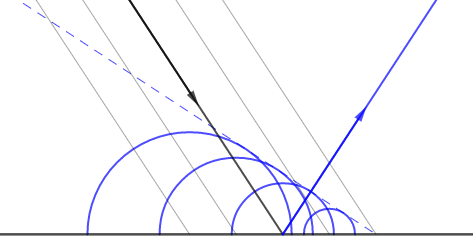
\includegraphics[width=0.45\linewidth]{figs/huygens_reflection.png}\hfill
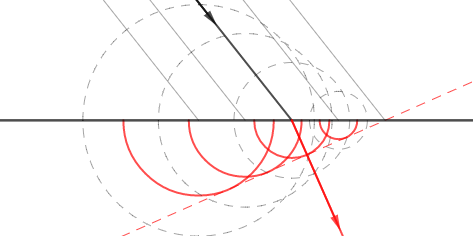
\includegraphics[width=0.45\linewidth]{figs/huygens_refraction.png}
\end{center}
\caption{Contruções geométricas para compreender, nos termos do princípio de
Huygens, a reflexão (esquerda) e a refração (direita) da luz. As linhas retas a
tracejado representam o envelope das ondas esféricas
secundárias.\label{fig:f060}}
\end{figure}

O Princípio de Huygens é fácil de compreender nos termos da interferência das
ondas secundárias produzidas em cada ponto de uma frente de onda. Ao mesmo
tempo, é muito útil para compreender os fenómenos que envolvem a interferência.
Voltaremos a este assunto no Capítulo~\ref{chpt:superp}, quando estudarmos a
sobreposição de ondas.


\newpage
\section{Introdução às ondas --- Resumo}
\begin{itemize}
\item
    Função de onda de ondas harmónicas unidimensionais:
    \begin{align*}
      \psi(x,t)&=A\cos\left(2\pi\left[\frac{x}{\lambda}\pm\frac{t}{T}\right]+
                \varphi_0\right)
               =A\cos\left(kx-\omega t-\varphi_0\right)\stackrel{!}{=}
               Ae^{\iu (kx-\omega t+\varphi_0)}
    \end{align*}
    com
    \begin{center}
    \begin{tabular}{c|l|l|l}
    \hline
    \rule{0mm}{3ex} Símbolo&Nome&Dimensões&Significado\\[0.5ex]
    \hline
    $A$ & Amplitude & Depende&
        \parbox[t]{0.3\textwidth}{\rule{0mm}{4ex}Módulo dos desvios máxi\-mos
        relativamente ao valor médio}\\
    $\lambda$ & Comprimento de onda & Comprimento &
        \parbox[t]{0.3\textwidth}{\rule{0mm}{4ex}Distância entre máximos da função
        de onda sucessivos} \\
    $T$ & Período & Tempo &
        \parbox[t]{0.3\textwidth}{\rule{0mm}{4ex}Intervalo de tempo entre a
        passagem, num ponto fixo, de dois máximos da função de onda sucessivos}
    \\
    $\varphi_0$&Constante de fase&Adimensional&
        \parbox[t]{0.3\textwidth}{\rule{0mm}{4ex}Fase da função de onda na
        origem do sistema de coordenadas, no instante $t=0$}\\
    $k$&Vetor de onda&
        \parbox[t]{0.2\textwidth}{Inverso do comprimento}&
        \parbox[t]{0.3\textwidth}{\rule{0mm}{4ex}Taxa espacial de variação da fase,
        expressa em $\text{rad}/\text{m}$}\\
    $\omega$&Frequência angular &
        \parbox[t]{0.2\textwidth}{Inverso do tempo}&
        \parbox[t]{0.3\textwidth}{\rule{0mm}{4ex}Taxa temporal de variação da
        fase, expressa em rad/s}
        \\
        &Fase& Adimensional &\parbox[t]{0.3\textwidth}{\rule{0mm}{4ex}%
          Argumento da função trigonométrica ou exponencial}
    \\[3ex]
    \hline
    \end{tabular}
    \end{center}
  \item Frequência: $f=1/T$. Unidades: ciclos por segundo ou Hz (hertz);
    representa a taxa temporal de variação da fase, expressa em ciclos por
    segundo.
    \begin{align*}
      f&=\frac{1}{T}&\omega&=\frac{2\pi}{T}&k&=\frac{2\pi}{\lambda}
    \end{align*}
\item Velocidade de propagação de uma onda harmónica:
\begin{equation*}
v=\frac{\lambda}{T}=\lambda f=\lambda \omega/2\pi=\frac\omega k
\end{equation*}
\item Ondas planas em 3D:
  \begin{align*}
    \psi(\vec r,t)&=A\cos(\vec k\cdot \vec r-\omega t+\varphi_0)\stackrel{!}{=}
                  A\e^{\iu(\vec k\cdot \vec r-\omega t+\varphi_0)}
  \end{align*}
  O vetor de onda $\vec k$ tem a direção e o sentido da propagação da onda. O
  seu módulo é $k=\|\vec k\|=2\pi/\lambda$.
\item
    Ondas esféricas em 3D:
    \begin{equation*}
    \psi(\vec r,t)=\frac{A}{r}\cos(kr-\omega t+\varphi_0)\stackrel{!}{=}
    \frac{A}{r}e^{\iu(kr-\omega t+\varphi_0)}
    \end{equation*}

\end{itemize}

